\documentclass[../m136main.tex]{subfiles}
\graphicspath{{\subfix{../figures/}}}

\begin{document}

\chapter{Analytic Functions}
\section{Limits and Differentiability}
Now we'll begin our study of functions $f : \C \to \C$, with the aim of mimicking the key results from calculus.

\begin{definition}[Limit]
    We say that $\ds \lim_{z \to z_0} f(z) = w_0$ if, for all $\varepsilon > 0$, there exists a $\delta > 0$ such that \vspace{-6pt}
    \[ 0 < |z - z_0| < \delta \;\implies\; |f(z) - w_0| < \varepsilon. \]
\end{definition}

That is, for every radius-$\varepsilon$ neighborhood around $w_0$, there is a radius-$\delta$ neighborhood around $z_0$ such that all $z$ in the $z_0$-neighborhood have $f(z)$ in the $w_0$-neighborhood.
We'll take all the basic limit properties as given, as their proofs are analogous to those in multivariable calculus.

\begin{definition}[Continuity]
    We say $f(z)$ is continuous at $z_0$ if
    \[ \lim_{z \to z_0} f(z) = f(z_0). \]
    $f$ is continuous on a set $\Omega$ if $f$ is continuous at each $z_0 \in \Omega$.
\end{definition}

Now, since the output of $f$ has real and imaginary parts, we must be able to write $f$ in the form
\[ f(x + iy) = u(x,y) + i \, v(x,y), \]
where $u,v : \R^2 \to \R$; in this case we write $u = \Re(f)$ and $v = \Im(f)$.
Conveniently, $f$ is continuous if and only if $u$ and $v$ are continuous at $(x_0, y_0)$!
We'll once again take all the basic continuity properties as given.

\begin{definition}[Derivative]
    Suppose $f(z)$ is defined in a neighborhood of $z_0 \in \C$.
    The derivative of $f$ at $z_0$ is
    \[ f'(z_0) = \lim_{z \to z_0} \frac{f(z) - f(z_0)}{z - z_0} = \lim_{h \to 0} \frac{f(z_0 + h) - f(z_0)}{h}, \]
    provided this limit exists.
    Such an $f$ is said to be differentiable at $z_0$.
\end{definition}

Once again, all rules for differentiation in $\R$ apply to differentiation in $\C$.
Note that $f$ is not necessarily differentiable if $\Re(f)$ and $\Im(f)$ are differentiable!

\begin{definition}[Analytic]
    A function $f$ is analytic (or holomorphic) on an open set $\Omega$ if $f$ is differentiable at each $z_0 \in \Omega$.
    $f$ is analytic at $z_0$ if there exists a neighborhood of $z_0$ on which $f$ is analytic, and if $f$ is analytic on $\C$ we say $f$ is entire.
\end{definition}

Analytic functions have a nice relationship between the transformations they represent and their derivatives.
From the definition we have the approximation
\[ f(z_0 + h) = f(z_0) + f'(z_0) h + \mathcal O (h), \]
meaning analytic functions are locally affine and $f'(z_0)$ encodes the information needed to take an small ``step'' away from $z_0$.
Such a step involves three kinds of transformations: a rotation, a dilation, and a translation.

Analytic functions are foundational to the study of the complex numbers.
They're characterized by a very particular relationship between their real and imaginary parts.

\begin{lemma}[]
    If $f = u + iv$ is differentiable at $z_0$ then
    \[ f'(z_0) = u_x + iv_x = v_y - i u_y. \]
\end{lemma}

\begin{proof}
    Suppose $f(x + iy) = u(x,y) + i \, v(x,y)$ is differentiable at $z_0 \in \C$, so the limit
    \[ f'(z_0) = \lim_{h \to 0} \frac{f(z_0 + h) - f(z_0)}{h} \]
    exists.
    If we approach along the horizontal axis (so $\Im(h) = 0$) and the vertical axis (so $\Re(h) = 0$) the limit becomes
    \[ f'(z_0) = \frac{\partial u}{\partial x}(x_0, y_0) + i \frac{\partial v}{\partial x}(x_0, y_0), \qquad f'(z_0) = -i \frac{\partial u}{\partial y}(x_0, y_0) + \frac{\partial v}{\partial y}(x_0, y_0) \]
    respectively.
    These expressions are equivalent.
\end{proof}

\begin{theorem}[Cauchy-Riemann equations]
    If $f = u + iv$ is differentiable at $z_0$ then \vspace{-8pt}
    \begin{align*}
        u_x &= \phantom{-}v_y, \\
        u_y &= -v_x.
    \end{align*}
    Consequently, if $f$ is analytic on an open set $\Omega$ then $f$ satisfies these equations everywhere in $\Omega$.
\end{theorem}

Notice that if the Cauchy-Riemann equations hold then we have the derivative matrix
\[ D \mbf{f} = \begin{bmatrix} u_x & u_y \\ v_x & v_y \end{bmatrix} = \begin{bmatrix} u_x & -v_x \\ v_x & u_x \end{bmatrix}, \]
which we recognize as a rotation-dilation matrix!
Now, we can see that satisfying the Cauchy-Riemann equations is a necessary condition for differentiability, but they are only one part of a sufficient condition.

\begin{theorem}[Sufficient condition for differentiability]
    Let $f = u + iv$ be defined in an open set $\Omega$ containing $z_0 = x_0 + iy_0$.
    If the first partials of $u$ and $v$ exist on $\Omega$, are continuous at $(x_0,y_0)$, and satisfy the Cauchy-Riemann equations at $(x_0,y_0)$, then $f$ is differentiable at $z_0$.

    Consequently, if these conditions hold everywhere in $\Omega$ then $f$ is analytic on $\Omega$.
\end{theorem}

\begin{proof}
    Let $h = s + it$.
    We first break the difference quotient into real and imaginary parts,
    \[ \frac{f(z_0 + h) - f(z_0)}{h} = \left( \frac{u(z_0 + h) - u(z_0)}{h} \right) + i \left( \frac{v(z_0 + h) - v(z_0)}{h} \right), \]
    and look specifically at its real component:
    \begin{align*}
        \frac{u(z_0 + h) - u(z_0)}{h} &= \frac{1}{h} \left[ \Big( u(x_0 + s, \, y_0 + y) - u(x_0 + s, \, y_0) \Big) + \Big( u(x_0 + s, \, y_0) - u(x_0, y_0) \Big) \right]. \\
        \intertext{By the mean value theorem in $\R$, there exist $0 < \theta_1, \theta_2 < 1$ such that}
        &= \frac{1}{h} \left[ \frac{\partial u}{\partial y} (x_0 + s, \, y_0 + \theta_1 t)t + \frac{\partial u}{\partial x} (x_0 + \theta_2 s, \, y_0)s \right] \\
        &= \frac{t}{h} \frac{\partial u}{\partial y} (x_0 + s, \, y_0 + \theta_1 t) + \frac{s}{h} \frac{\partial u}{\partial x} (x_0 + \theta_2 s, \, y_0).
    \end{align*}
    We could go through an analogous line of reasoning to get a similar expression for the imaginary component.
    Adding the results gives
    \begin{align*}
        \frac{f(z_0 + h) - f(z_0)}{h} &= \frac{t}{h} \left[ \frac{\partial u}{\partial y} (x_0 + s, \, y_0 + \theta_1 t) + i \frac{\partial v}{\partial y} (x_0 + s, \, y_0 + \theta_3 t) \right] \\
        &\qquad\quad + \frac{s}{h} \left[ \frac{\partial u}{\partial x} (x_0 + \theta_2 s, \, y_0) + i \frac{\partial v}{\partial x} (x_0 + \theta_4 s, \, y_0) \right].
    \end{align*}
    We'd like to show that this expression approaches $f'(z_0)$ as $h \to 0$.
    To this end we subtract $\frac{s + it}{h} (u_x + i v_x)$ and show that the result goes to zero.
    Call the difference $\delta$, so
    \begin{align*}
        \delta &= \frac{t}{h} \Big[ u_y (x_0 + s, \, y_0 + \theta_1 t) + v_x(x_0, y_0) + i \Big( v_y(x_0 + s, \, y_0 + \theta_3 t) - u_x(x_0, y_0) \Big) \Big] \\
        &\qquad\quad + \frac{s}{h} \Big[ u_x(x_0 + \theta_2 s, \, y_0) - u_x(x_0, y_0) + i \Big( v_x(x_0 + \theta_4 s, \, y_0) - v_x(x_0, y_0) \Big) \Big].
    \end{align*}
    Applying the Cauchy-Riemann equations demonstrates that, if $u$ and $v$ are continuous, then $\delta \to 0$.
    Thus $f'(z_0)$ exists.
\end{proof}

\section{Harmonic Functions}
It turns out that analytic functions are deeply tied to the harmonic functions central to the study of PDEs!
We'll state the following a fun fact for now, deferring a proof to later.

\begin{theorem}[Harmonic conjugates]
    If $u + iv$ is analytic on a domain (an open and connected set) $\Omega$ then $\Delta u = \Delta v = 0$ on $\Omega$.
    In other words, $u$ and $v$ are harmonic functions.
    (In particular, because they are the real and imaginary parts of an analytic function, $u$ and $v$ are called harmonic conjugates.)
\end{theorem}

\begin{theorem}[]
    Harmonic conjugates have orthogonal level curves.
\end{theorem}

\begin{proof}
    Consider a level curve $u(x,y) = C$ with parametrization $\mbf{x}(t) = \big( x(t), y(t) \big)$.
    By the chain rule,
    \[ 0 = \frac{d}{dt} u \big( x(t), y(t) \big) = \frac{\partial u}{\partial x} x'(t) + \frac{\partial u}{\partial y} y'(t) = \nabla u \cdot \mbf{x}'(t), \]
    meaning $\nabla u$ is orthogonal to the level curves of $u$.
    Now, if $u,v$ are harmonic conjugates then by the Cauchy-Riemann equations $\nabla u \cdot \nabla v = (u_x, u_y) \cdot (v_x, v_y) = 0$.
    So when $\nabla u \neq 0 \neq \nabla v$, the level curves of $u$ and $v$ are orthogonal.
\end{proof}

Now for a nice application of harmonic functions that isn't explicitly related to complex variables, but is interesting nonetheless.

\pagebreak

\begin{theorem}[Mean-value property of harmonic functions]
    Let $B(z_0, r)$ denote be the closed ball of radius $r$ about $z_0$.
    If $\phi(x,y)$ is harmonic on the open set $\Omega \subseteq \R^2$ then
    \[ \phi(x_0, y_0) = \frac{1}{2\pi r} \int_{\partial B(z_0, r)} \phi(x,y) \,ds \]
    for any $r > 0$ such that $B(z_0, r) \subseteq \Omega$.
\end{theorem}

\begin{proof}
    The average value of $\phi$ over the boundary of $B(z_0, r)$ is
    \[ \frac{1}{2\pi r} \int_{\partial B(z_0, r)} \phi(x,y) \,ds = \frac{1}{2\pi r} \int_{0}^{2\pi} \phi(x_0 + r \cos t, \, y_0 + r  t) r \,dt. \]
    Differentiating:
    \begin{align*}
        \frac{dm}{dr} &= \frac{1}{2\pi r} \int_{0}^{2\pi} \left( \frac{\partial \phi}{\partial x} (x,y) \cdot r \cos t + \frac{\partial \phi}{\partial y} (x,y) \cdot r \sin t \right) dt \\
        &= \frac{1}{2\pi r} \int_{\partial B(z_0, r)} \nabla \phi \cdot \mbf{n} \,ds. \\
        \intertext{By the divergence theorem,}
        &= \frac{1}{2\pi r} \iint_{B(z_0, r)} \nabla \cdot (\nabla \phi) \, dA \\
        &= \frac{1}{2\pi r} \iint_{B(z_0, r)} \Delta \phi \, dA = 0.
    \end{align*}
    Thus $m(r)$ is independent of by $r$, and by continuity $\ds m(r) = \lim_{r \to 0} m(r) = \phi(x_0, y_0)$, as desired.
\end{proof}

\section{Exponential and Trigonometric Functions}
Now we'll look at a few particularly important analytic functions called elementary functions.

\begin{definition}[Complex exponential]
    If $z = x + iy$ then
    \[ e^{z} = e^{x} \cos y + i e^{x} \sin y. \]
\end{definition}

We can immediately make a few observations.
\begin{itemize}[topsep=0pt]
    \item The complex exponential agrees with the familiar real-valued exponential when evaluated on the real line, as we'd expect from a generalization to $\C$.
    \item $e^{z}$ is entire with derivative $e^{z}$, as we'd hope.
    \item The familiar $e^{x + iy} = e^{x} e^{iy}$ and $e^{z+w} = e^{z} e^{w}$ hold, meaning $e^{nz} = (e^{z})^{n}$ and $(e^{i\theta})^n = e^{in\theta}$ for $n \in \Z$.
    \item The magnitude of $e^{z}$ is determined entirely by the real part of its argument: $|e^{z}| = |e^{\Re z}|$.
    \item If $z = iy$ then $e^{iy} = \cos y + i \sin y$, meaning $r \cis \theta = r e^{i\theta}$!
    It follows that $e^{z}$ is $2\pi$-periodic parallel to the imaginary axis.
    \item $e^{z}$ and its components are harmonic.
\end{itemize}
From the definition we can also see that exponentiation maps vertical lines $z = x_0 + iy$ to radius-$e^{x_0}$ circles, and horizontal lines $z = x + iy_0$ to rays going off in the direction of $e^{iy_0}$.

\begin{center}
    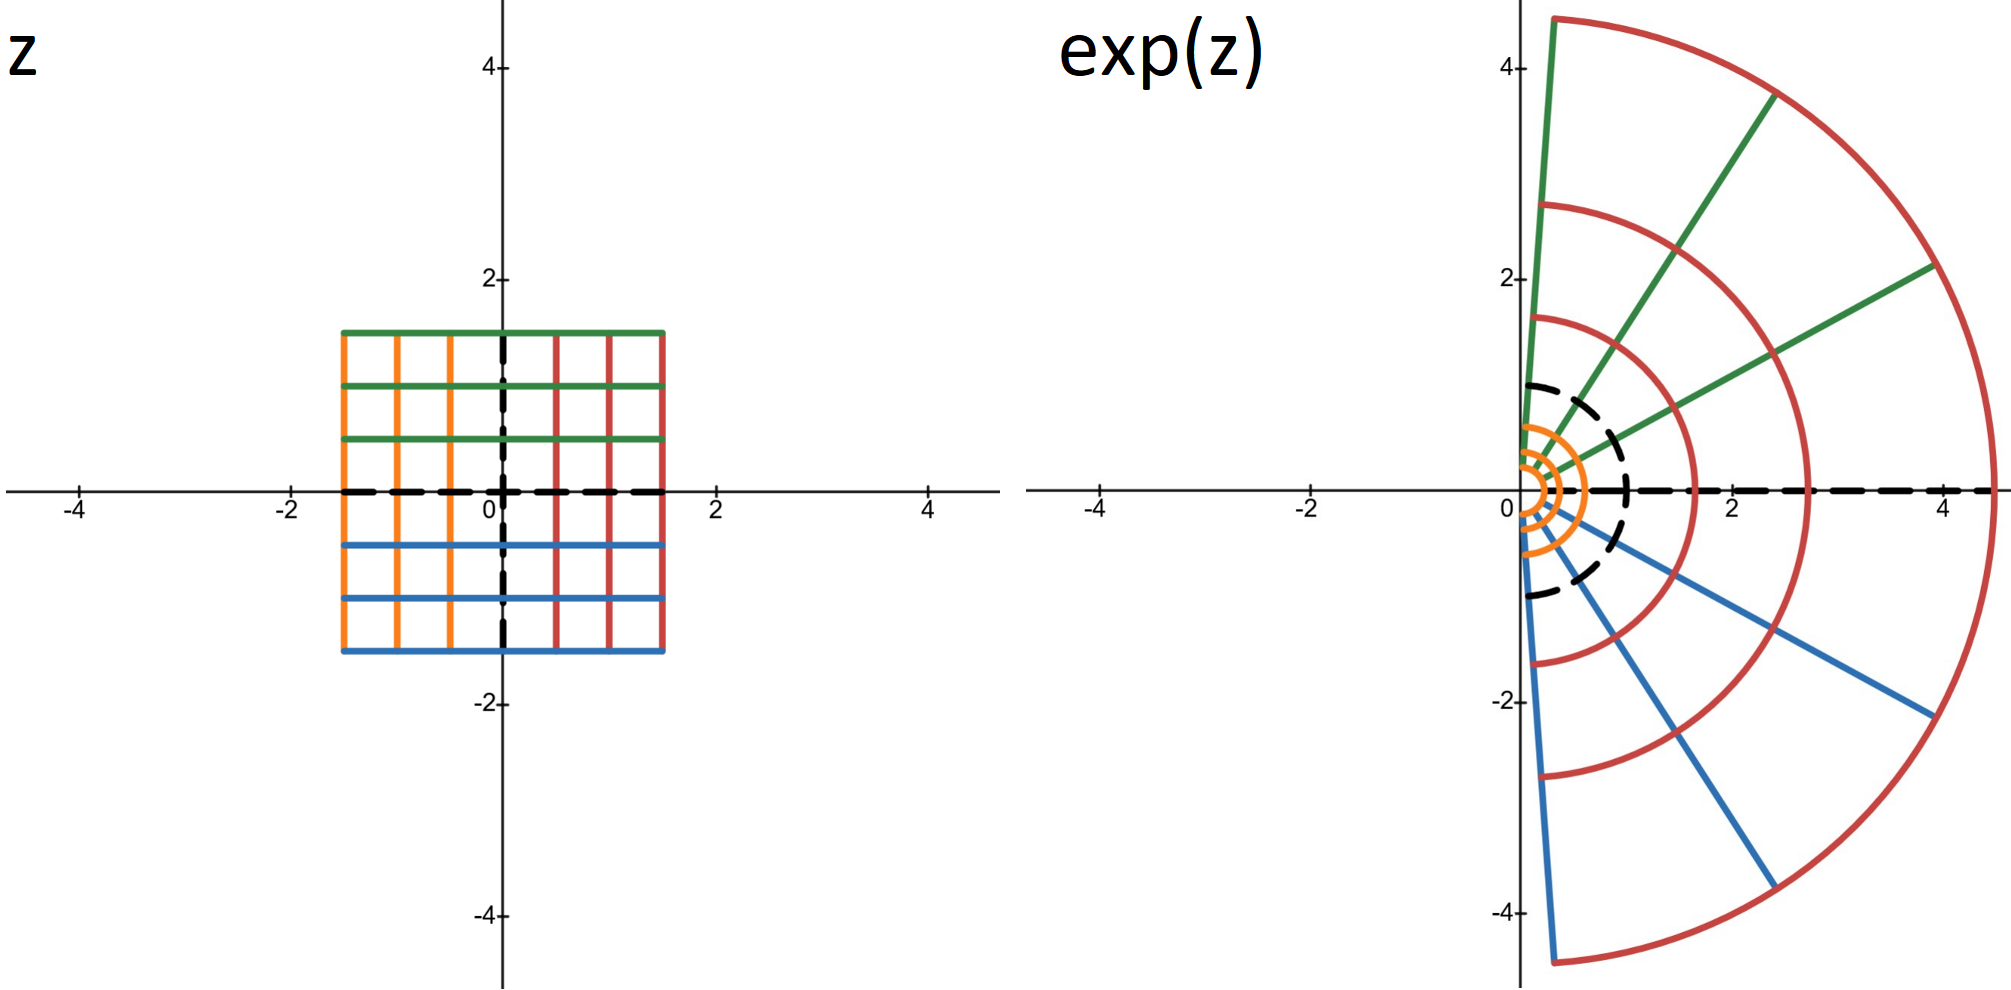
\includegraphics[width=0.75\textwidth]{exponential.png}
\end{center}

Now we'll use Euler's formula $e^{i\theta} = \cos \theta + i \sin \theta$ to define the complex sine and cosine.

\begin{definition}[Complex sine and cosine]
    If $z \in \C$ then
    \[ \cos z = \frac{e^{iz} + e^{-iz}}{2}, \qquad \sin z = \frac{e^{iz} - e^{-iz}}{2i}. \]
\end{definition}

We'll once again make some observations.
\begin{itemize}[topsep=0pt]
    \item Both sine and cosine agree with their real-valued counterparts when evaluated on the real line.
    \item $\sin z$ and $\cos z$ are entire with derivatives $\cos z$ and $-\sin z$, respectively.
    \item The familiar trigonometric identities hold: $\sin(-z) = -\sin z$, $\cos(-z) = \cos z$, $\sin^2 z + \cos^2 z = 1$,
    \begin{align*}
        \sin(z + w) &= \sin z \cos w + \cos z \sin w, \\
        \cos(z + w) &= \cos z \cos w - \sin z \sin z.
    \end{align*}
    \item The real and imaginary parts of each function are
    \begin{align*}
        \Re [\sin z] &= \sin x \cosh y, & \Re [\cos z] &= \phantom{-}\cos x \cosh y, \\
        \Im [\sin z] &= \cos x \sinh y, & \Im [\cos z] &= -\sin x \sinh y.
    \end{align*}
\end{itemize}
Let's take a quick look at sine.
If we define $u = \sin x \cosh y$ and $v = \cos x \sinh y$ then we can write
\[ \frac{u^2}{\cosh^2 y} + \frac{v^2}{\sinh^2 y} = 1, \qquad \frac{u^2}{\sin^2 x} - \frac{v^2}{\cos^2 x} = 1. \]
Thus horizontal lines at $y_0$ map to ellipses and vertical lines at $x_0$ map to half-hyperbolas.
(For $0 < x_0 < \pi$ we get a right-hyperbola, while for $\pi < x_0 < 2\pi$ we get a left-hyperbola.)

Finally, note that we define the complex hyperbolic trig functions in the exact same way as the real ones.

\section{Logarithms and Power Functions}
In defining the complex logarithm we must keep in mind that we should have $\log z = w$ if and only if $e^{w} = z$.
We can see that if $w = u + iv$ then
\[ e^{u} = |z|, \qquad v = \arg z. \]
Thus the logarithm must be a multi-valued function---although we can guarantee $e^{\log z} = z$ for all admissible $z$, in general we must write $\log e^{z} = z + 2\pi i k$ for all $k \in \Z$.
The definition follows.

\pagebreak

\begin{definition}[Complex logarithm]
    If $z \in \C \setminus \left\{ 0 \right\}$, define the set- and single-valued functions
    \begin{align*}
        \log z &= \ln |z| + i \arg(z), \\
        \Log z &= \ln |z| + i \Arg(z).
    \end{align*}
    We will continue to write $\ln x$ for the real function $\ln x = \int_{1}^{x} dt / t$.
\end{definition}

\begin{theorem}[Logarithms are analytic]
    The function $\Log z$ is analytic on all of $\C$, excluding the non-positive real axis; for such $z$,
    \[ \frac{d}{dz} \Log z = \frac{1}{z}. \]
    It follows that the real part $\frac{1}{2} \ln (x^2 + y^2)$ is harmonic.
\end{theorem}

\begin{proof}
    Let $w = \Log z$ and $w_0 = \Log z_0$.
    We know, from properties of the exponential function, that
    \[ \lim_{w \to w_0} \frac{z - z_0}{w - w_0} = \frac{dz}{dw} \Big|_{w = w_0} = e^{w_0} = z_0. \]
    Note that $w \to w_0$ as $z \to z_0$ and that $w \neq w_0$ as long as $z \neq z_0$.
    Thus
    \[ \lim_{z \to z_0} \frac{w - w_0}{z - z_0} = \lim_{w \to w_0} \frac{1}{\frac{z - z_0}{w - w_0}} = \frac{1}{z_0}, \]
    as desired.
\end{proof}

We can see that we must treat the non-positive real axis carefully while working with the principal logarithm.
But really, there's nothing special about this axis---we could easily have defined the single-valued logarithm a different way and gotten a different ray to be careful of.

\begin{definition}[Branch]
    $F(z)$ is a branch of the multi-valued $f(z)$ on a domain $D$ if $F(z)$ is single-valued and continuous on $\Omega$, and for each $z \in \Omega$, $F(z)$ is one of the values $f(z)$.
    The set of points at which $F(z)$ is continuous is called the branch cut of $F$.
\end{definition}

With this in mind, we call $\Log z$ the principal branch of the logarithm; the non-positive real axis is its branch cut.
A branch with analytic range $(\theta, \theta + 2\pi]$ is denoted by $\Log_\theta z$ (with argument $\Arg_\theta z$), and its branch cut is in the direction of $e^{i \theta}$.
The branch we choose to work with depends primarily on where we want the branch cut to be---or, rather, where we don't want it to be.

We can use logarithms to define power functions involving complex numbers!

\begin{definition}[Power function]
    Let $z \in \C \setminus \left\{ 0 \right\}$ and $\alpha \in \C$.
    Then
    \[ z^{\alpha} = e^{\alpha \log z}. \]
\end{definition}

Power functions are generally multi-valued, but not always---note that
\[ z^{\alpha} = e^{\alpha \ln |z| + i\alpha \Arg z} e^{i \cdot 2\pi \alpha k}, \]
so for real $\alpha$ we have three cases.
If $\alpha \in \Z$ then $e^{i \cdot 2\pi \alpha k} = 1$ for all $k$ and $z^{\alpha}$ is single-valued; if $\alpha \in \Q$ then the $e^{i \cdot 2\pi \alpha k}$ are evenly spaced around the unit circle; and for irrational $\alpha$ the exponential $e^{i \cdot 2\pi \alpha k}$ fills the unit circle densely.

We choose a branch of $z^{\alpha}$ by picking out a branch of the logarithm, so the principal branch is
\[ z^{\alpha} = e^{\alpha \Log z} \]
with the branch cut along the non-positive real axis.
Off the branch cut we have
\[ \frac{d}{dz} z^{\alpha} = \frac{d}{dz} e^{\alpha \Log z} = \frac{\alpha}{z} e^{\alpha \Log z} = \alpha z^{\alpha - 1}. \]
A couple more notes.
First, the familiar laws of exponents hold---multiplication turns into addition, and division into subtraction.
We can also use out brief analysis of power functions to determine when we're allowed to split (principal) square roots like $\sqrt{z^2} = \sqrt{z} \sqrt{z}$!
Following the definition, we can see that
\[ \sqrt{z^2} = e^{\ln |z|} e^{i \frac{1}{2} \Arg (z^2)}, \qquad \sqrt{z} \sqrt{z} = e^{\ln |z|} e^{i \Arg z}. \]
For equality we require $\Arg z^2 = 2 \Arg z$, so we must have $\Arg z \in (-\pi / 2, \pi / 2]$.
In other words, these are the $z$ for which squaring doesn't move its argument outside the principal branch!

\end{document}